\newpage
\chapter*{Simulations}
\addcontentsline{toc}{chapter}{Simulations} 




% Reconsider later if some if this is better placed in methods section
% or under different title
\section*{Frictional properties of the intact graphene sheet}
The friction measurment simulation is governed by the following parameters, which is divided into three sub categories for the purpose of this thesis as shown in table \ref{tab:param}.



\begin{table}[H]
  \begin{center}
  \caption{Parameters of the numerical procedure for measuring friction.}
  \label{tab:param}
  \begin{tabular}{ | c | m{8cm}| m{5cm}|} 
    \hline
    Category & Parameter name: description & Category purpose \\ 
    \hline
    Physical & 
    \begin{itemize}
      \item[-] T: Temperature for the Langevin thermostat.
      \item[-] $v_{drag}$: Drag speed for the sheet translation.
    \end{itemize} &
    Parameters that we expect to have an inevitably effect on the system friction properties, for which the choice will be a baseline for our studies.
    \\ \hline
    Measurement & 
    \begin{itemize}
      \item[-] $dt$: Integration timestep.
      \item[-] $t_R$: Relaxtion time before strething.
      \item[-] Pauses between stretch and adding normal force and between dragging the sheet.  
      \item[-] Stretch Speed: How fast to stretch the sheet.
      \item[-] $K$: Spring constant for the spring responsible of translating the sheet. An infinte spring constant is achieved by moving the end blocks as a rigid body (Lammps: fix move).
      \item[-] Drag Length: How far to translate the sheet.
      \item[-] Sheet size: Spatial size of the 2D sheet.  
    \end{itemize} &
    Paramters that effects the simulation dynamics and the 'experimental procedure' that we a mimicking. We aim to choose to these paramters such that the friction properties is stable for small perturbations.  \\ \hline
    ML input & 
    \begin{itemize}
      \item[-] Sheet configuration: A binary matrix containing information of which atoms is removed (0) and which is still present (1) in the graphene structure.
      \item[-] Scan angle: The direction for which we translate the sheet.
      \item[-] Stretch amount: The relative sheet stretch in percentage.
      \item[-] $F_N$: Applied normal force to the end blocks.
    \end{itemize} &
    The ramaining paramters that serve as the governing variables in the optimization process for certain friction properties and is thus the input variables for the ML part. 
    \\ \hline
  \end{tabular}
  \end{center}
\end{table}


We should try to set the physcis and measurement parameters in such a way that we reduce computation speed where it is doesn't infer with the frictional properties study.

We need to define some ranges for the ML input paramters. $F_N$, stretch ranges where it is not prone to ruptures. The configuration it self does not have clear rules but is also being regulated by the no rupture requirement. 

\newpage
\subsection{Baseline}

\subsubsection{Looking at the friction data}

\begin{figure}[H]
  \centering
  \begin{subfigure}[b]{0.49\textwidth}
      \centering
      \includegraphics[width=\textwidth]{figures/baseline/drag_Ff_10Å.pdf}
      \caption{Drag length of 10 Å}
      \label{fig:drag_Ff_10}
  \end{subfigure}
  \hfill
  \begin{subfigure}[b]{0.49\textwidth}
      \centering
      \includegraphics[width=\textwidth]{figures/baseline/drag_Ff_100Å.pdf}
      \caption{Drag length of 100 Å}
      \label{fig:drag_Ff_100}
  \end{subfigure}
  \hfill
     \caption{Friction force $F_\parallel$ between (full) sheet and substrate with respect to the drag direction vs drag length. Drag length is measured by the constant movement of the virtual atom and not the COM of the sheet. The red line represents a savgol filter with window length 150 (corresponding to a drag length of 3 Å or a time window of 15 ps) and polyorder 5. }
     \label{fig:drag_Ff}
\end{figure}

From figure \ref{fig:drag_Ff} we observe that the friction force measured parallel to the drag direction fluctates with a wavelike pattern. By performing a fourier transform of the data we can idendity some of the leading frequencies as seen in figure \ref{fig:ft}. We can clearly see how the frequencies of $0.0395$/Å and $0.028$/Å fits well with some of the slower oscillations in the data. The faster oscialltions is more changelling to idendity and we did not attempt to match with any sine wave here. 


\begin{figure}[H]
  \centering
  \begin{subfigure}[b]{0.49\textwidth}
      \centering
      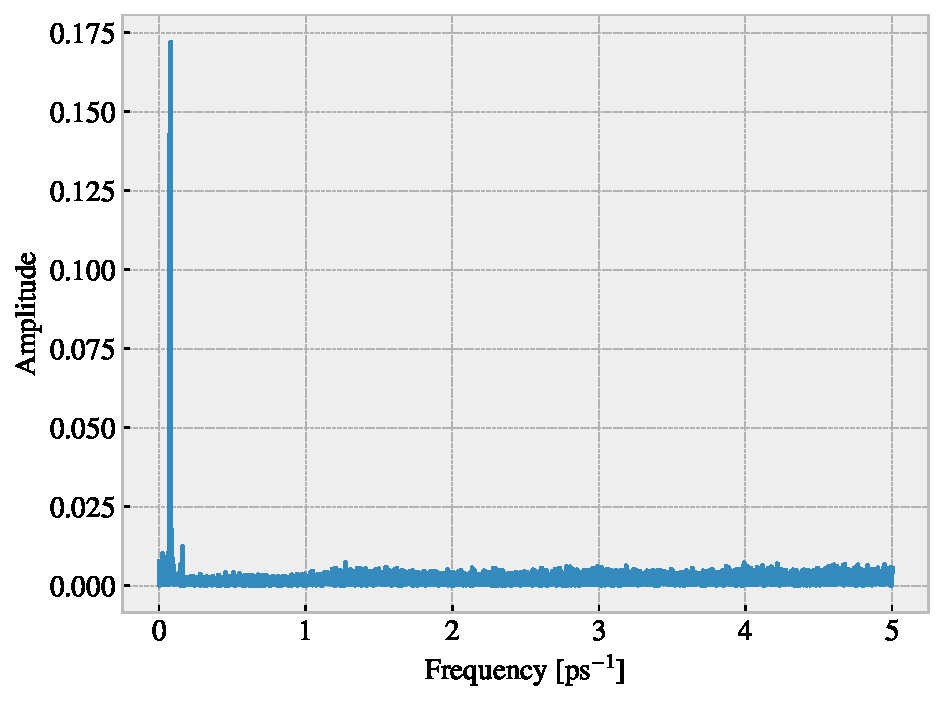
\includegraphics[width=\textwidth]{figures/baseline/ft.pdf}
      \caption{Full frequency range.}
      \label{fig:ft_a}
  \end{subfigure}
  \hfill
  \begin{subfigure}[b]{0.49\textwidth}
      \centering
      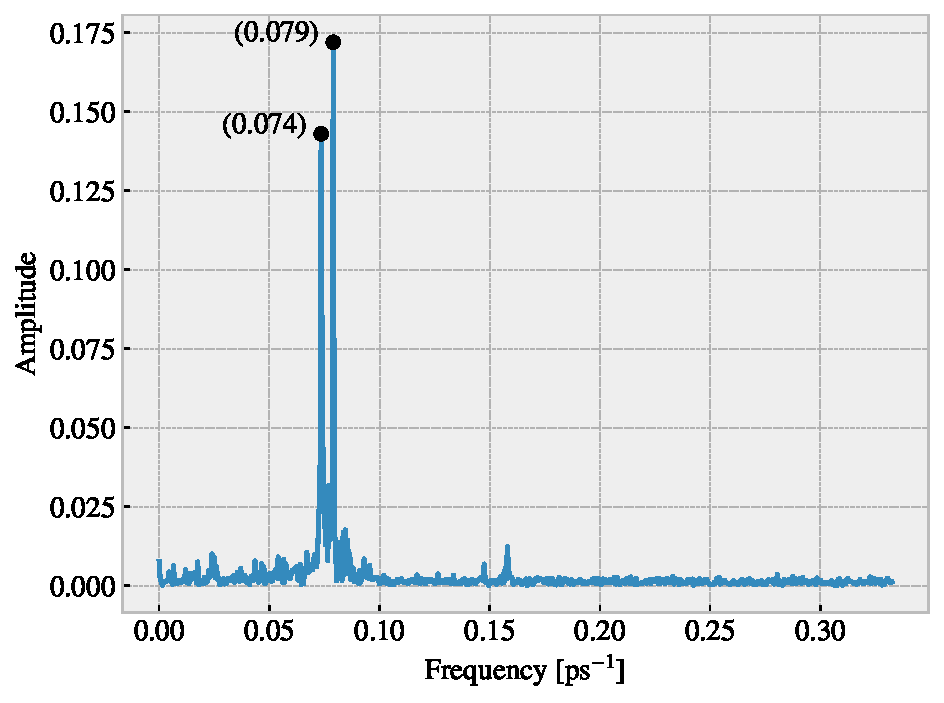
\includegraphics[width=\textwidth]{figures/baseline/ft_zoom.pdf}
      \caption{Reduced frequency range.}
      \label{fig:ft_b}
  \end{subfigure}
  \hfill
  \begin{subfigure}[b]{0.49\textwidth}
      \centering
      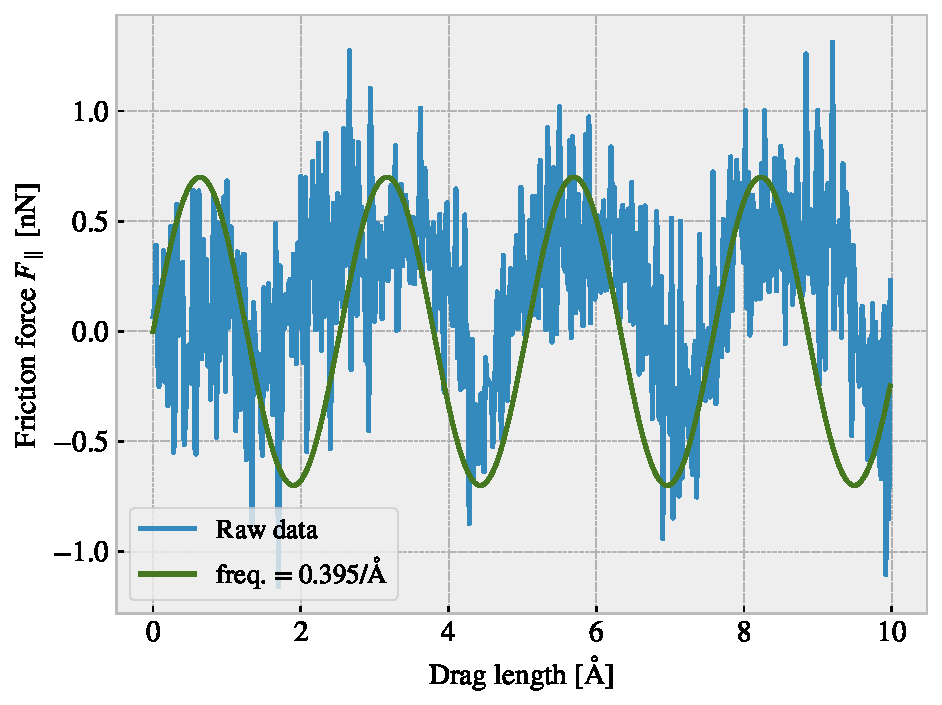
\includegraphics[width=\textwidth]{figures/baseline/ft_sine_zoom.pdf}
      \caption{Selected frequencies applied to data from figure \ref{fig:drag_Ff_10}}
      \label{fig:ft_c}
  \end{subfigure}
  \hfill
  \begin{subfigure}[b]{0.49\textwidth}
      \centering
      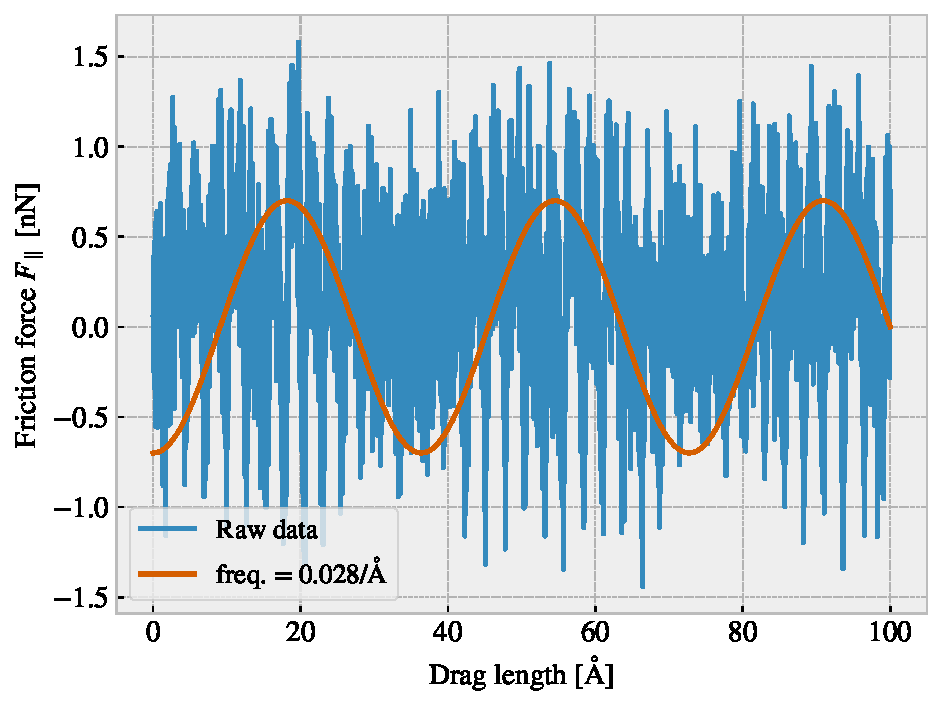
\includegraphics[width=\textwidth]{figures/baseline/ft_sine.pdf}
      \caption{Selected frequencies applied to data from figure \ref{fig:drag_Ff_100}}
      \label{fig:ft_d}
  \end{subfigure}
  \hfill
     \caption{Fourier transform on data shown in figure \ref{fig:drag_Ff}.}
     \label{fig:ft}
\end{figure}


Decompositions. \\
It is tempting to only look at the friction force on the sheet since this is where we apply cuts. Any desired effect taking place here in contrast to the untouched Pull blocks can be scaled by simply increasing the size of the sheet. However as we see (in some of the figures hopefully) the distribution of force acting on the pull block and the sheet vary back and forth. Thus we cannot ignore effects of force distribution which can be induced by certain cut patterns. 

What about the full sheet vs norm discussion. Are we better of just taking the full norm?

I guess the conclusion is that the para/perp decomposition show that these are easily seperateable + it gives a plus minus axis instead of having a friction norm. When the sheet moves backwards this should count negatively I think. For the sheet/PB decomposition we see that the pattern is not as clean when we seperate them and thus we are better off keeping the full sheet measurement.

\begin{figure}[H]
  \centering
  \begin{subfigure}[b]{0.49\textwidth}
      \centering
      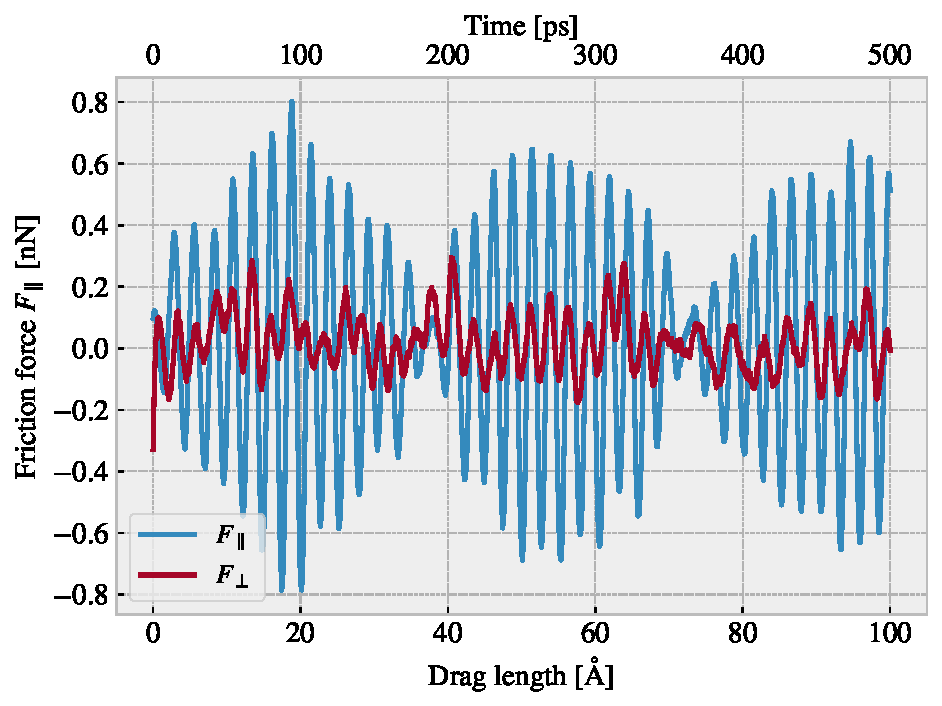
\includegraphics[width=\textwidth]{figures/baseline/decomp_direc.pdf}
      \caption{Decomposition into parallel ($\parallel$) and perpendicular $(\perp)$ to drag direction}
      \label{fig:decomp_direc}
  \end{subfigure}
  \hfill
  \begin{subfigure}[b]{0.49\textwidth}
      \centering
      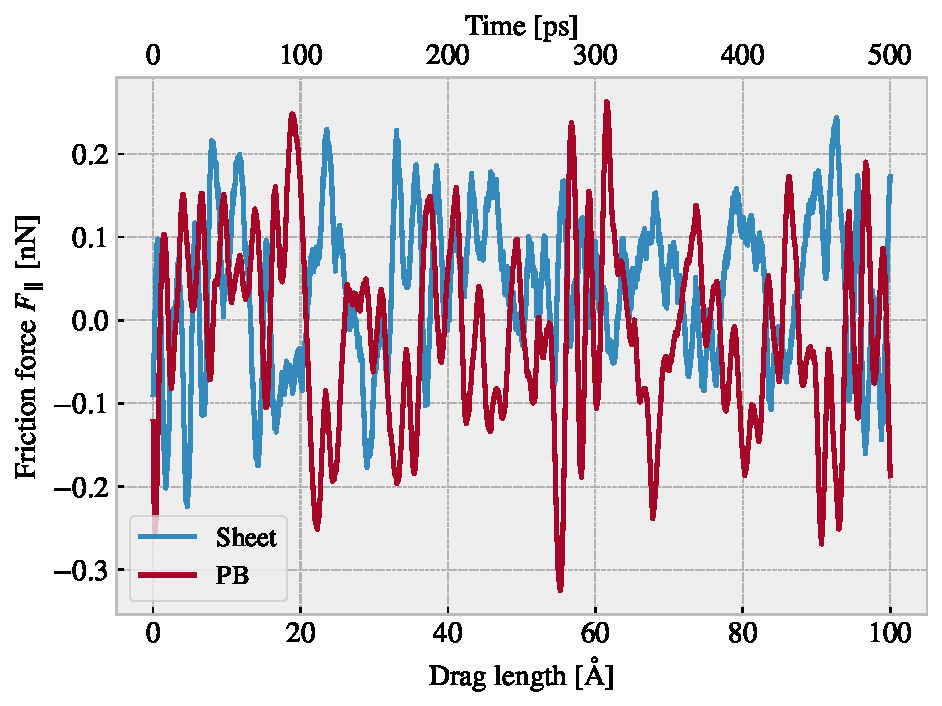
\includegraphics[width=\textwidth]{figures/baseline/decomp_group.pdf}
      \caption{Decomposition into group inner sheet (sheet) and pull blocks (PB).}
      \label{fig:decomp_group}
  \end{subfigure}
  \hfill
     \caption{Decompostion of friction force.}
     \label{fig:decomp}
\end{figure}


Look at the COM path.

\begin{figure}[H]
  \centering
  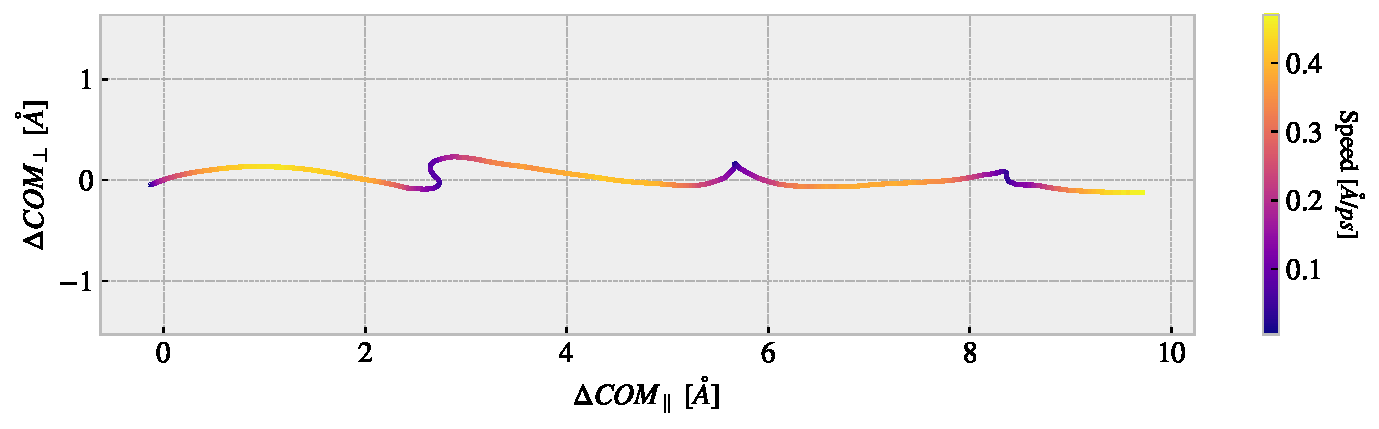
\includegraphics[width=\linewidth]{figures/baseline/COM_path.pdf}
  \caption{...}
  \label{fig:COM_path}
\end{figure}


Should we plot some contact graphs here also? They are really not interesting until we get to the stretch part. I thik we should include there as a tool for measuring the change of the sheet when stretching.

\subsubsection{Defining single metrics with uncertainty}

We are interested in defining single metrics that describe the frictional properties of the sheet. A naturall reference point is the dynamic and static friction coefficient. We can represent these as the mean and max friction force value respectively, but we leave the division by normal force for now as it is only a factor. 


\begin{figure}[H]
  \centering
  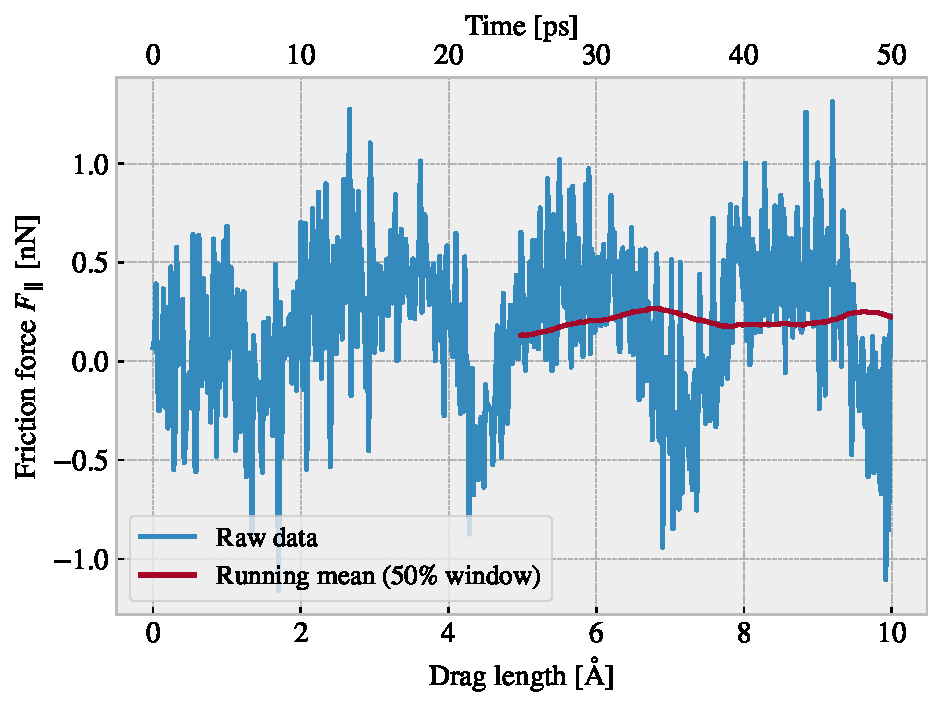
\includegraphics[width=0.7\linewidth]{figures/baseline/Ff_running_mean.pdf}
  \caption{...}
  \label{fig:Ff_runmean}
\end{figure}


A way to quanity the uncertainy of the mean friction evaluation is by looking at the running mean score shown in figure \ref{fig:Ff_runmean}. If the running mean is constant we know that it doesn't really matter whether we stop now to measure or if we drag it a bit longer. However, any fluctuations of this line means that out mean measurement is still sensitive to the drag length. We should not care for flucations in the beginning of the running mean curve as this is essentially including data from the rough beginning transistioning from static to dynamic friction. Only the running mean close to the ending should be considered for our uncertainty. One way is to take then standard deviation in the final 20\% of the running mean curve as a way of approximation the unceetainty of the final mean value. This is shown in figure \ref{fig:Ff_runstd}. 

\begin{figure}[H]
  \centering
  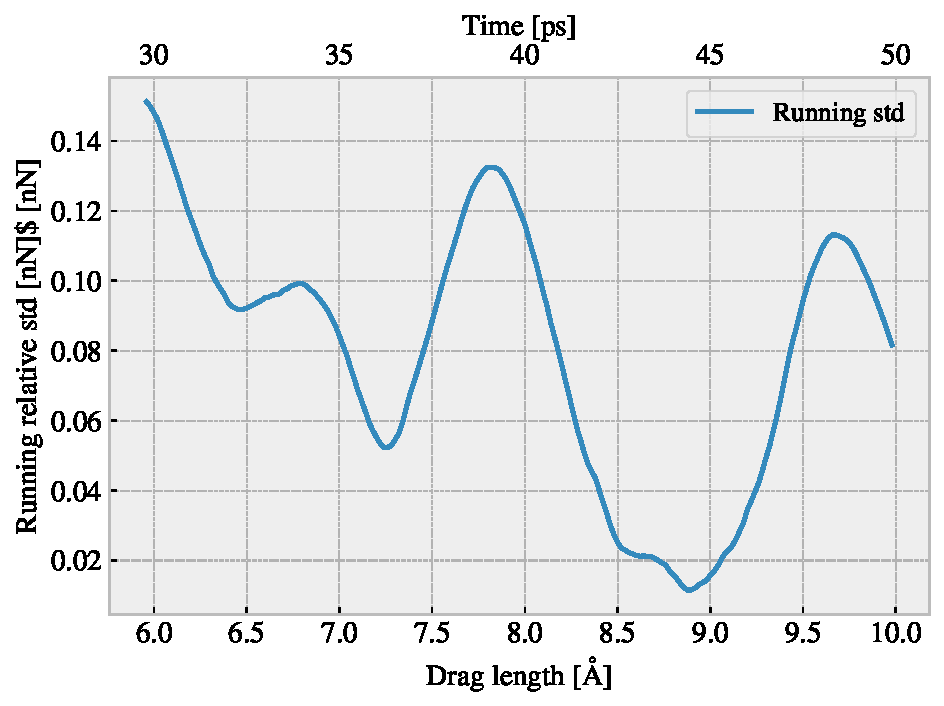
\includegraphics[width=0.7\linewidth]{figures/baseline/Ff_running_std.pdf}
  \caption{Running std (window 20\%) on runmean from figure \ref{fig:Ff_runmean} divided by mean of each window. }
  \label{fig:Ff_runstd}
\end{figure}

From figure \ref{fig:Ff_runstd} we can see that the this provides us with an uncertainty at 8\% relative error when stopping at drag length 10 Å. We also notice that stopping a bit earlier seemed to give better results which reflects the more stable looking part of the running mean roughly between drag length 8 Å and 9 Å. By dragging it for a total of 400 Å we get a final uncertainty of about 3.5 \%. The choice of window size for these running evaluations is somewhat abitrary and thus we should not really trust the exact numric value of the uncertainty, but it serves as an indication of the fluctuations that we are going to pick up in our metrics which we eventually are going to pass on to neural network as true labels. \\

For the max value we do not really have a good way to determine the uncertainty...


\subsubsection{Varying normal force and stretch}

Show multi plot results with uncertainty bars. 


\subsubsection(Varying temperature, drag speed, spring constant and dt)

\begin{figure}[H]
  \centering
  \begin{subfigure}[b]{0.49\textwidth}
      \centering
      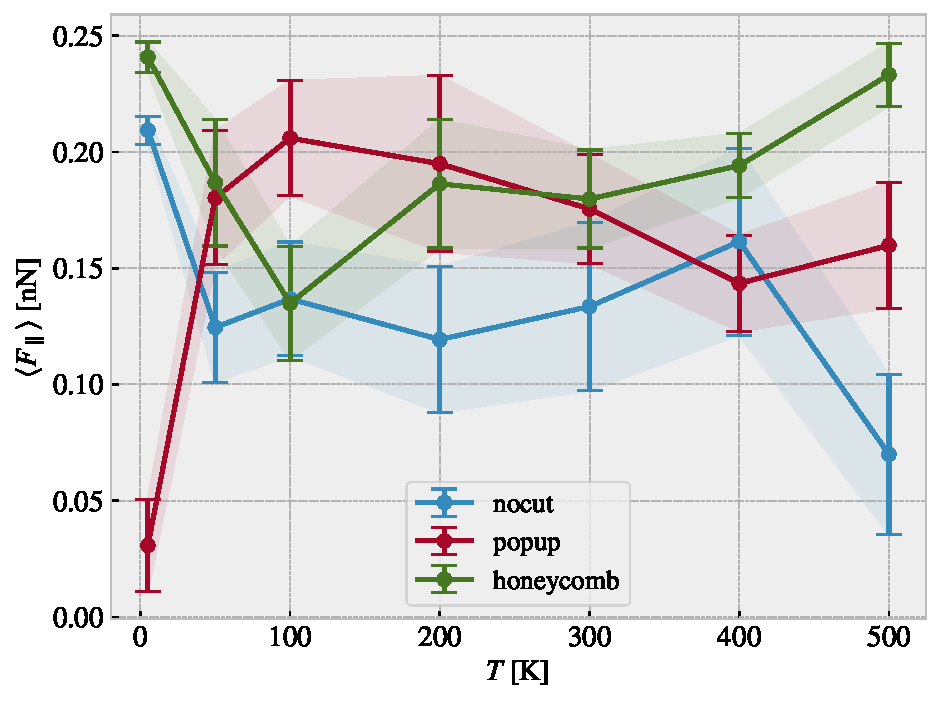
\includegraphics[width=\textwidth]{figures/baseline/variables_temp_mean.pdf}
      \caption{mean friction}
      \label{fig:var_temp_mean}
  \end{subfigure}
  \hfill
  \begin{subfigure}[b]{0.49\textwidth}
      \centering
      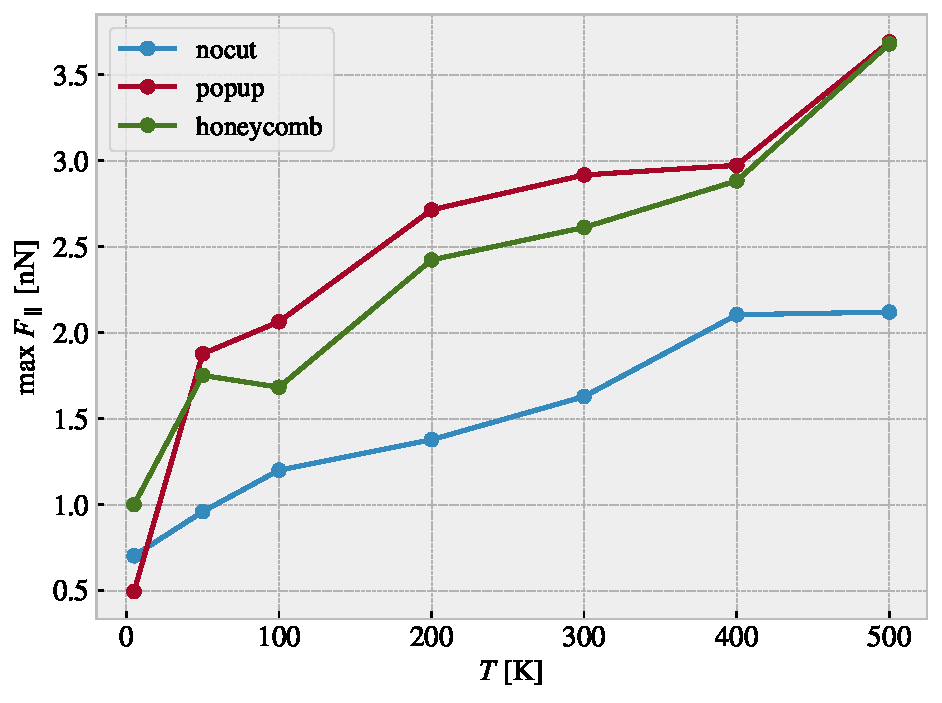
\includegraphics[width=\textwidth]{figures/baseline/variables_temp_max.pdf}
      \caption{max friction}
      \label{fig:var_temp_max}
  \end{subfigure}
  \hfill
     \caption{Temperature}
     \label{fig:var_temp}
\end{figure}

\begin{figure}[H]
  \centering
  \begin{subfigure}[b]{0.49\textwidth}
      \centering
      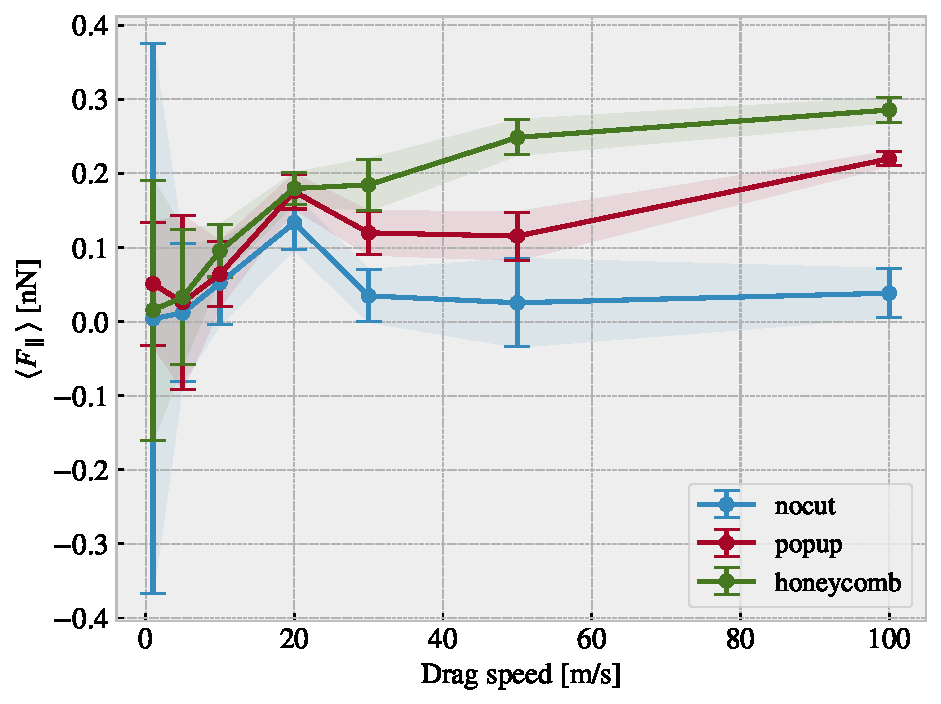
\includegraphics[width=\textwidth]{figures/baseline/variables_vel_mean.pdf}
      \caption{mean friction}
      \label{fig:var_vel_mean}
  \end{subfigure}
  \hfill
  \begin{subfigure}[b]{0.49\textwidth}
      \centering
      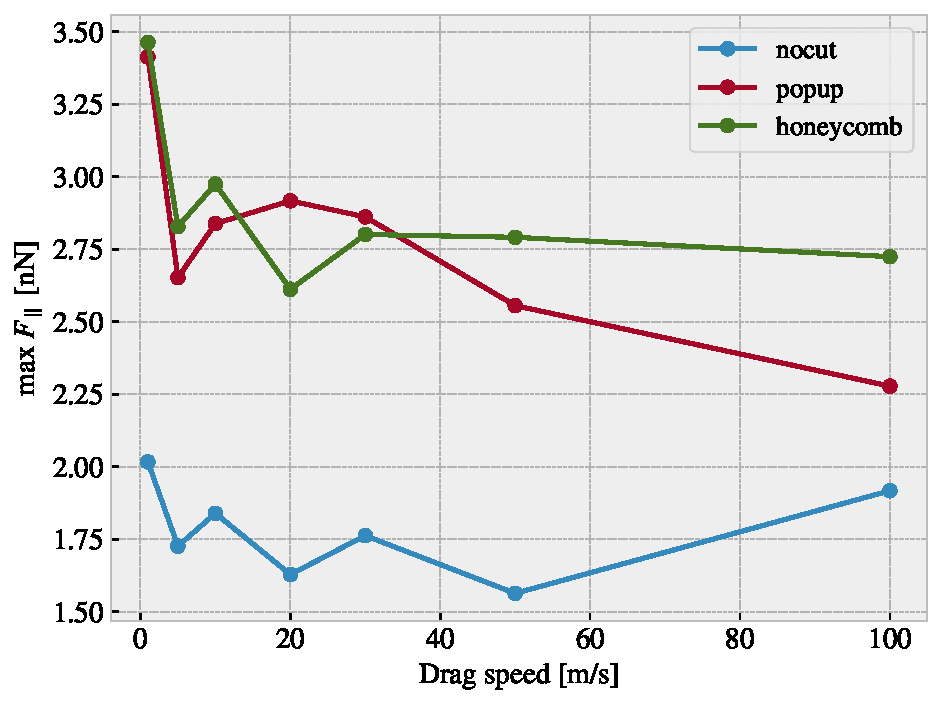
\includegraphics[width=\textwidth]{figures/baseline/variables_vel_max.pdf}
      \caption{max friction}
      \label{fig:var_vel_max}
  \end{subfigure}
  \hfill
     \caption{Drag speed}
     \label{fig:var_vel}
\end{figure}

\begin{figure}[H]
  \centering
  \begin{subfigure}[b]{0.49\textwidth}
      \centering
      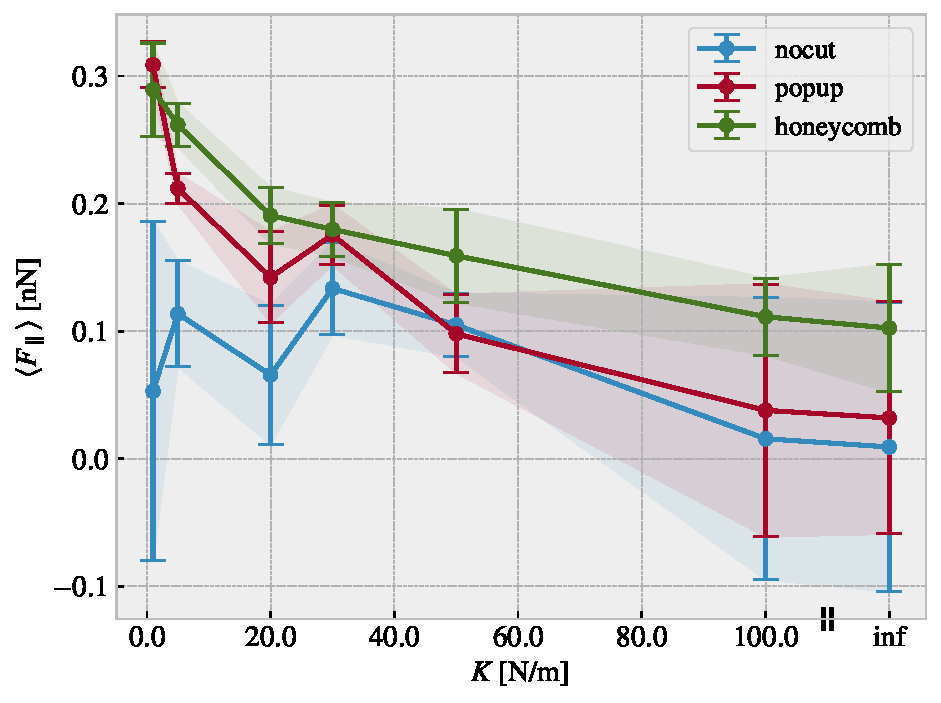
\includegraphics[width=\textwidth]{figures/baseline/variables_spring_mean.pdf}
      \caption{mean friction}
      \label{fig:var_K_mean}
  \end{subfigure}
  \hfill
  \begin{subfigure}[b]{0.49\textwidth}
      \centering
      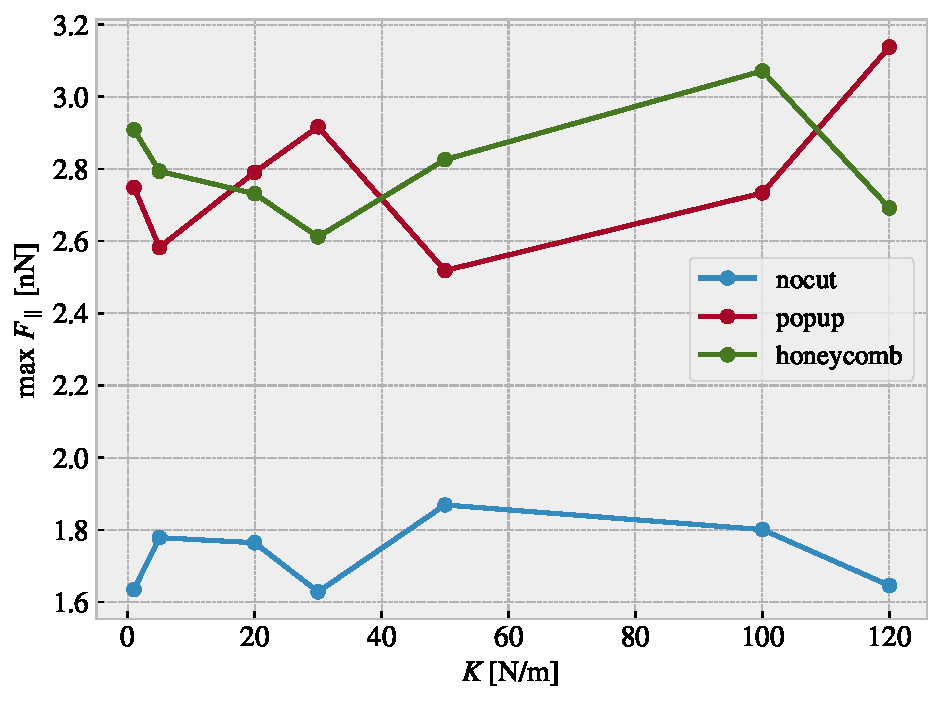
\includegraphics[width=\textwidth]{figures/baseline/variables_spring_max.pdf}
      \caption{max friction}
      \label{fig:var_K_max}
  \end{subfigure}
  \hfill
     \caption{Spring constant}
     \label{fig:var_K}
\end{figure}

\begin{figure}[H]
  \centering
  \begin{subfigure}[b]{0.49\textwidth}
      \centering
      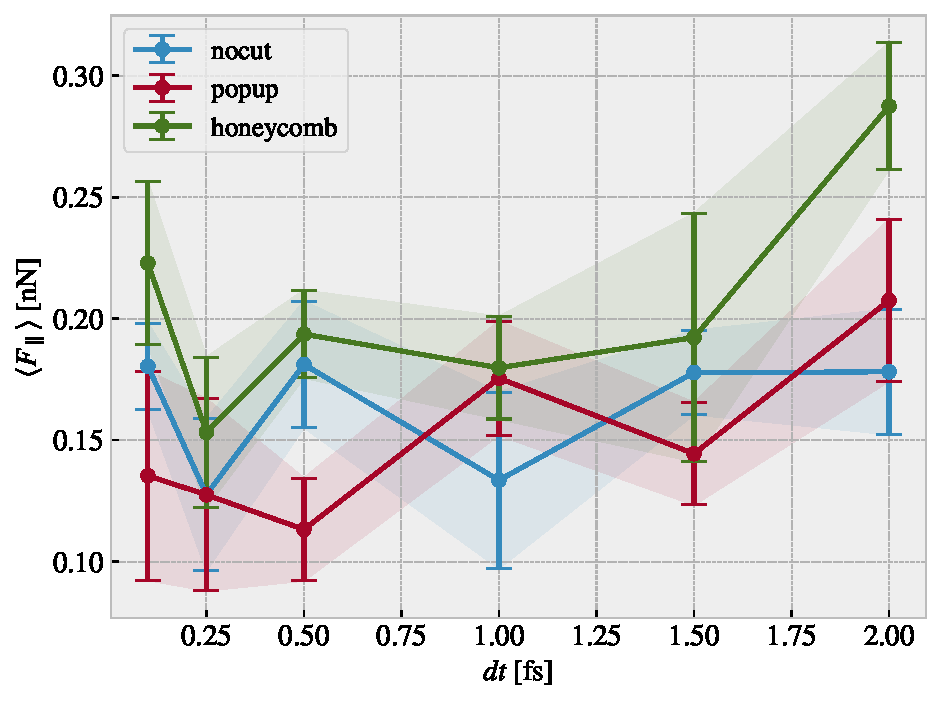
\includegraphics[width=\textwidth]{figures/baseline/variables_dt_mean.pdf}
      \caption{mean friction}
      \label{fig:var_dt_mean}
  \end{subfigure}
  \hfill
  \begin{subfigure}[b]{0.49\textwidth}
      \centering
      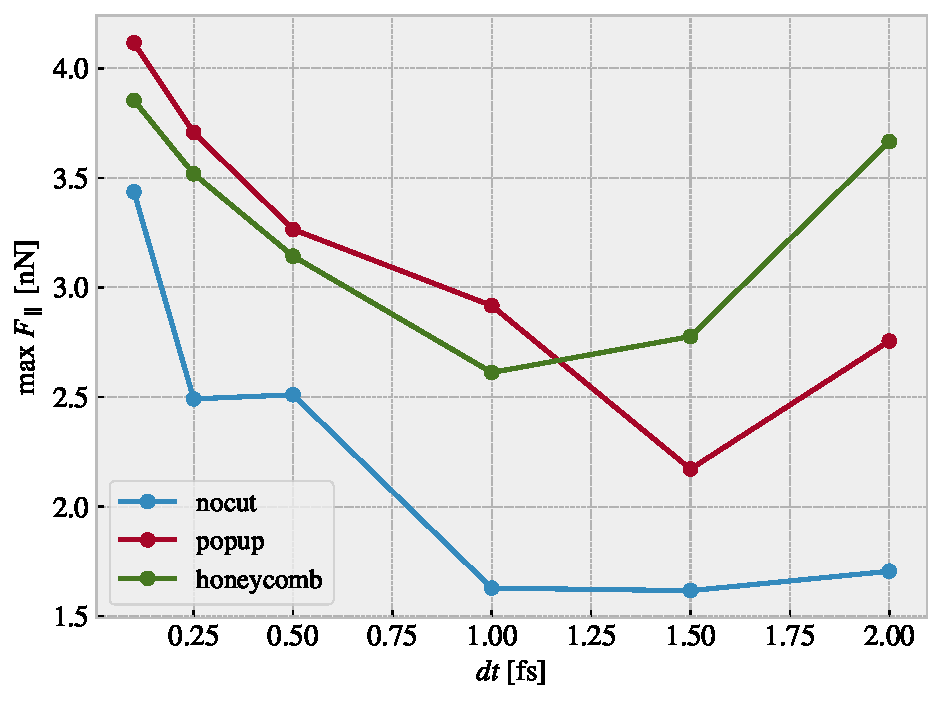
\includegraphics[width=\textwidth]{figures/baseline/variables_dt_max.pdf}
      \caption{max friction}
      \label{fig:var_dt_max}
  \end{subfigure}
  \hfill
     \caption{Timestep}
     \label{fig:var_dt}
\end{figure}

Multi stretch 



\begin{figure}[H]
  \centering
  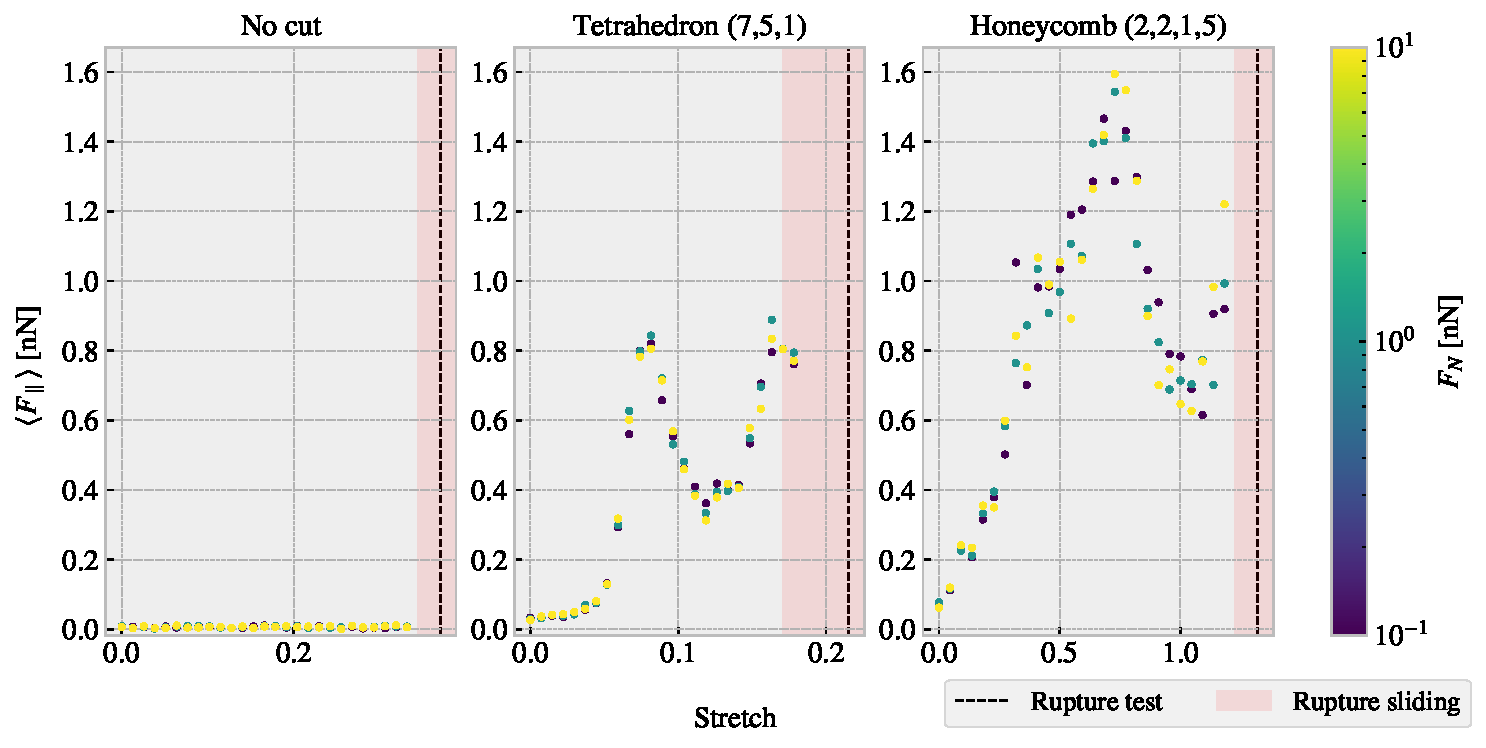
\includegraphics[width=\linewidth]{figures/baseline/multi_stretch_mean_compare.pdf}
  \caption{...}
  \label{fig:}
\end{figure}


\begin{figure}[H]
  \centering
  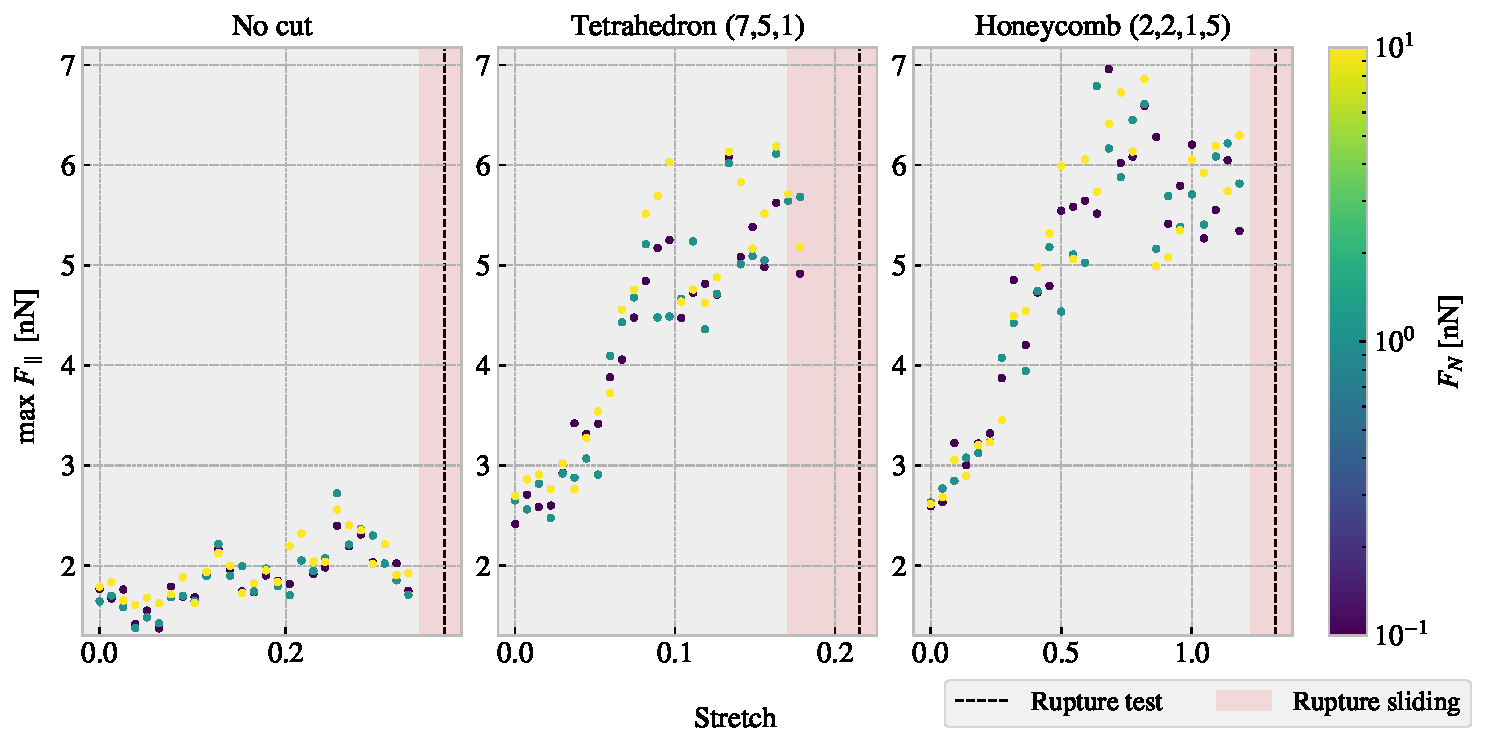
\includegraphics[width=\linewidth]{figures/baseline/multi_stretch_max_compare.pdf}
  \caption{...}
  \label{fig:}
\end{figure}



\newpage
\subsection*{Observations}



\begin{itemize}
  \item stretch $= 0$ \% and $F_N = 188$ eV/Å yielded a very small amount of wear (two atoms visually out of place), for which the sheet dug into the substrate when passing by the second time. For the same normal force but 0.25 \% this problem did not occour. We need to stay out of the friction wear regime. Amorphic substrate is even more prone to this problem of wear.
\end{itemize}